\chapter{Results}

This chapter evaluates the system in two settings: \emph{offline} on the held-out part of the InSDN dataset, and \emph{live} in the Mininet laboratory where real attacks are generated against a running SDN and the system must stop them. The evaluation is organised around the following questions.

\begin{itemize}
	\item What aspects of the system are evaluated?
		\begin{itemize}
			\item Detection quality of the GNN: is a window an attack, which type, and which host is the attacker (the questions that correspond to FR4--FR5 and NFR2).
			\item Whether a graph model is better than flow-level models trained on the same features (the central hypothesis of the project).
			\item Inference latency of the complete service path (NFR1).
			\item Effectiveness and safety of automated mitigation in a real SDN (FR9--FR13, NFR3, NFR4): the fraction of attack traffic dropped, the time to mitigate and the collateral damage to benign hosts.
		\end{itemize}
\end{itemize}

\begin{enumerate}[label=\Roman*]
	\item \textbf{Cases of comparison.} Random Forest and XGBoost (flow-level, results aggregated per window) against the GAT (Table~\ref{tab:main}); GAT against GCN, GraphSAGE, GAT without edge features and two other window sizes (Table~\ref{tab:ablation}); the InSDN-only model against the model fine-tuned on laboratory traffic (Table~\ref{tab:finetune}); eight feature-selection and reduction methods against the full feature set (Table~\ref{tab:featsel}); and four successive versions of the mitigation logic (Table~\ref{tab:mitigation}).
	\item \textbf{Performance metrics.} Window F1, false-positive rate (FPR) and ROC-AUC measure whether an attack is detected and how often benign traffic is flagged; macro-F1 over the major attack classes measures the attack-type decision (classes with fewer than 20 test windows are reported separately because one window decides their F1); host F1, precision and recall measure the attacker identification; the p50/p90/p99 latency measures real-time suitability; the drop rate, time to mitigation, and the number of runs with a benign host blocked measure the mitigation. Accuracy alone is not used because the benign class is 38\% of the test windows and the attack classes are very unequal in size.
\end{enumerate}

\begin{enumerate}
	\item \textbf{Parameters under study.} Convolution type (GAT, GCN, GraphSAGE), use of edge features, window size (50, 100, 200 flows), feature subset, and in the live system the confirmation windows, host-score aggregation (maximum or mean), rate-limit units (kbit/s or packets/s) and rule priorities.
	\item \textbf{Experimental setup.} Described in Section~\ref{sec:testenv}. Hyper-parameters: hidden size 64, 4 attention heads, 2 layers, dropout 0.2, AdamW \cite{bib:adam} with learning rate $10^{-3}$, weight decay $10^{-4}$, batch size 64, gradient clipping at norm 2.0 and a learning-rate scheduler that halves the rate after 5 epochs without improvement, up to 60 epochs with patience 10, seed 42. They are the default values for a model of this size (about $6\times10^4$ parameters, on 12,458 training windows); the values were fixed in the configuration file before the final runs and the variants that were compared are in the ablation study.
\end{enumerate}

\section{Test Set up Environment}
\label{sec:testenv}

\begin{table}[htbp]
\centering
\caption{Test environment}
\label{tab:env}
\small
\begin{tabularx}{\textwidth}{|p{3.4cm}|X|}
\hline
\textbf{Item} & \textbf{Description} \\ \hline
Machine & Laptop, Arch Linux (kernel 6.19), NVIDIA GeForce RTX 3050 Laptop GPU; the same machine hosts the IDS and the Docker laboratory \\ \hline
Software & Python 3.14.3, PyTorch 2.11, PyTorch Geometric 2.7, scikit-learn 1.8, XGBoost 3.2, FastAPI \\ \hline
Input (offline) & Cleaned InSDN CSV files (343,888 flows) converted to 17,780 windows of 100 flows: 12,458 training, 2,645 validation and 2,677 test windows (time-ordered split) \\ \hline
Input (live) & Mininet topology: 2 OpenFlow~1.3 Open vSwitch switches and 6 hosts (2 attackers, 1 web server that is also the victim, 3 benign clients); benign traffic (web polling by three clients and an iperf3 stream) runs throughout; attacks are generated with hping3 and nmap \\ \hline
Controller / IDS & os-ken application polling every 2~s, IDS window 10~s, ATTACK threshold 0.85, confirmation in 2 consecutive windows, rule timeouts 60~s idle and 300~s hard \\ \hline
Outputs & JSON result files and plots in \texttt{results/phase2/}, audit log \texttt{mitigation\_log.jsonl}, ground-truth JSON and pcap per live run \\ \hline
Evaluation of live runs & Each run: 25~s benign, 45~s attack, 40~s benign. Three runs for each of DDoS, DoS, Probe and BruteForce (12 attack runs) plus benign-only runs. A run is split between training and test as a whole when collecting lab data. \\ \hline
\end{tabularx}
\end{table}

The dataset is highly imbalanced in the minor classes. After the time-ordered split, the test windows are: Benign 1,025, DDoS 731, DoS 322, Probe 588, BruteForce 9, WebAttack 1 and Botnet 1.

\begin{figure}[htbp]
\centering
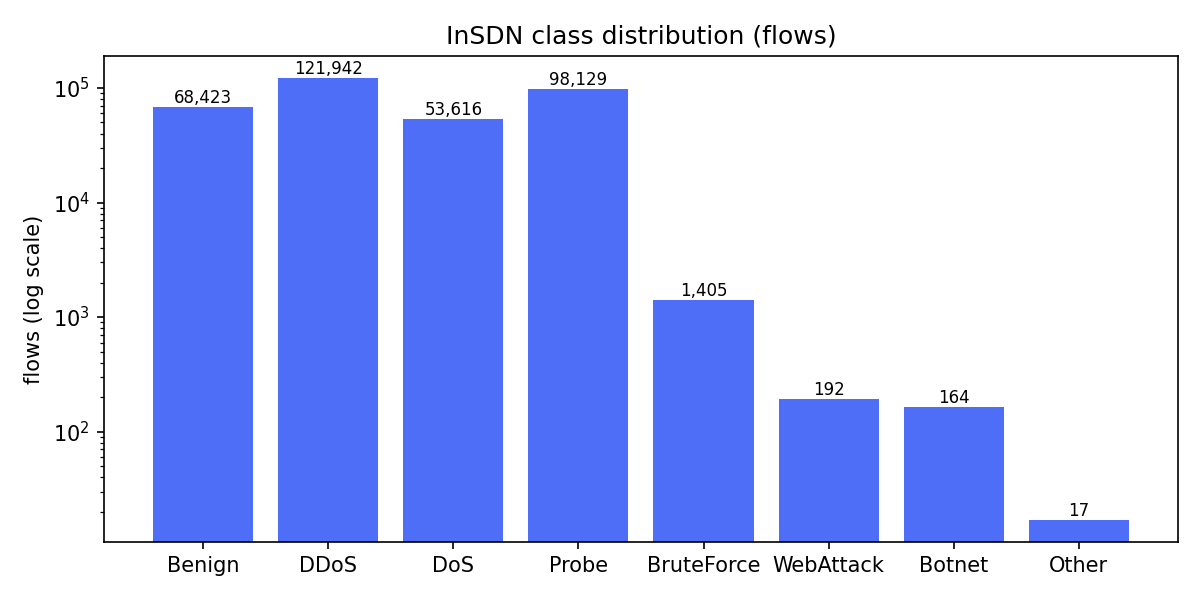
\includegraphics[width=0.9\textwidth]{class_distribution}
\caption{Class distribution of the InSDN flows used in the graphs}
\label{fig:classdist}
\end{figure}

\section{Test Procedures and Test Cases}

All test cases are automated unless stated otherwise. The automated test suite (\texttt{pytest}, 45 tests) passes completely and covers preprocessing and label mapping, graph construction and the split gap, the live feature path, and the Mininet tools.

\begin{longtable}{|p{1.2cm}|p{2.6cm}|p{3.1cm}|p{3.6cm}|p{3.0cm}|}
\caption{Test cases}\label{tab:tc}\\
\hline
\textbf{ID} & \textbf{Requirement} & \textbf{Pre-condition and procedure} & \textbf{Expected result} & \textbf{Actual result} \\ \hline
\endfirsthead
\hline \textbf{ID} & \textbf{Requirement} & \textbf{Pre-condition and procedure} & \textbf{Expected result} & \textbf{Actual result} \\ \hline
\endhead
TC-01 & FR1 (normal) & Raw InSDN files; run cleaning and label mapping & Benign rows labelled Benign; unknown labels become Other & Pass: 68,423 \texttt{Normal} rows kept as Benign (Phase~1 had labelled them as attacks); automated tests pass \\ \hline
TC-02 & FR2 (normal) & Compute features for sample records & 16 edge and 16 node features with the defined meaning & Pass (unit tests) \\ \hline
TC-03 & FR2, NFR8 (normal) & Compare features from the dataset path with those from the live collector for the same records & Identical values & Pass (live-path tests) \\ \hline
TC-04 & FR3 (robustness) & Build windows with overlap and split & No flow appears in two splits; every class present in every split & Pass (unit test of the gap) \\ \hline
TC-05 & FR4, FR5 (normal) & Train GAT, RF and XGBoost on the same split; evaluate on test windows & Window F1 $>0.95$, FPR $<5\%$ & Pass: F1 0.9985, FPR 0 (Table~\ref{tab:main}) \\ \hline
TC-06 & FR5 (comparison) & Train GCN, GraphSAGE, no-edge GAT and window 50/200 variants & Results for every variant & Done (Table~\ref{tab:ablation}) \\ \hline
TC-07 & FR5 (comparison) & Run feature-selection comparison on edge and node tables & Comparison for each method and $k$; a selected subset & Done (Table~\ref{tab:featsel}) \\ \hline
TC-08 & FR4 (robustness) & Evaluate rare classes (BruteForce, WebAttack, Botnet) & Behaviour reported and explained & GAT fails on WebAttack and Botnet (1 test window each) and BruteForce (9); see analysis \\ \hline
TC-09 & FR6, NFR1 (normal) & Export TorchScript; compare with eager model on 100 graphs; measure latency per window size & Identical outputs; p99 $<50$~ms for typical windows & Pass: identical; p99 9.6~ms (CPU service path) \\ \hline
TC-10 & FR7, FR8 (normal) & Replay held-out flows as OpenFlow statistics through the live pipeline (benign $\to$ attack $\to$ benign) & Attack windows flagged, benign not & Pass: all attack windows flagged; 0 false alerts in 55 benign windows (Table~\ref{tab:replay}) \\ \hline
TC-11 & NFR1 (stress) & Latency with 100 to 5,000 records per window on CPU and GPU & Below 50~ms & Pass: p99 $\le$ 24.4~ms up to 2,000 records on CPU; at 5,000 records 41.0~ms on GPU and 52.3~ms on CPU (slightly above the target) \\ \hline
TC-12 & FR9, NFR4 (abnormal) & Benign-only live runs & No rule installed & Pass: 0 rules in benign-only runs \\ \hline
TC-13 & FR9, FR13, NFR3 (normal) & 12 live attack runs (3 per attack type) & At least 70\% attack traffic dropped & Pass: 12/12 runs, mean 94.7\% (Table~\ref{tab:mitigation}) \\ \hline
TC-14 & FR13 (normal) & Measure time from attack start to the first rule & Reported & Mean 7.5~s, p90 17.2~s; median 4.5~s \\ \hline
TC-15 & FR9, NFR4 (robustness) & Check that no benign host is blocked in any attack run; whitelisted hosts never blocked & No false blocks & Pass: 0 runs with a benign host blocked in the final system; whitelist applied in the alert classifier \\ \hline
TC-16 & FR12, NFR5, NFR10 (normal, manual) & Open \texttt{/}, \texttt{/live}, \texttt{/pipeline} during a live demo; use block/unblock with and without the API key & Pages show data; mutating calls rejected without key & Verified manually during demonstrations (screenshots in Figures~\ref{fig:shot-offline}--\ref{fig:shot-live}) \\ \hline
TC-17 & NFR6, NFR8 (normal) & Run the complete pytest suite & All tests pass & Pass: 45 passed \\ \hline
\end{longtable}

\section{Snapshots}

\subsection{Phase 1 model and the effect of the data leakage}

The first model of the project (Phase 1) built graphs from random windows. Its test F1 of 0.994 fell to 0.983 when the same model was evaluated on a time-ordered split (Table~\ref{tab:leak}): random splits of overlapping windows put near-identical windows into both sets. All later results therefore use the time-ordered split. The Phase 1 graphs also had no real topology (the CICIDS2017 variant used has no IP addresses), so they were replaced by the InSDN host graphs.

\begin{table}[htbp]
\centering
\caption{Effect of the split on the Phase 1 model}
\label{tab:leak}
\begin{tabular}{|l|c|c|c|c|}
\hline
\textbf{Split} & \textbf{Test F1} & \textbf{Precision} & \textbf{Recall} & \textbf{ROC-AUC} \\ \hline
Random (Phase 1) & 0.9940 & 0.9950 & 0.9930 & -- \\ \hline
Time-ordered & 0.9826 & 1.0000 & 0.9659 & 0.9961 \\ \hline
\end{tabular}
\end{table}

\subsection{GAT versus the baselines}

\begin{table}[htbp]
\centering
\caption{Comparison on the InSDN test split (2,677 windows). Macro-F1 (major) is over Benign, DDoS, DoS and Probe.}
\label{tab:main}
\small
\begin{tabular}{|l|c|c|c|c|c|c|}
\hline
\textbf{Model} & \textbf{Window F1} & \textbf{FPR} & \textbf{ROC-AUC} & \textbf{Macro-F1 (major)} & \textbf{Host F1} & \textbf{Host P / R} \\ \hline
Random Forest & 0.9976 & 0.0000 & 0.9987 & 0.9702 & 0.9941 & 0.9957 / 0.9925 \\ \hline
XGBoost & 0.9979 & 0.0000 & 0.9987 & 0.9703 & 0.9946 & 1.0000 / 0.9893 \\ \hline
\textbf{GAT-IDS} & \textbf{0.9985} & 0.0000 & 0.9982 & \textbf{0.9785} & \textbf{0.9975} & 0.9980 / 0.9971 \\ \hline
\end{tabular}
\end{table}

The baselines score each flow and aggregate the flow scores of a window; their host scores come from a model that receives the same per-host features as the GAT. Window-level binary detection is already saturated for all three models (F1 above 0.997 and no false positives). The graph model gives its gain on the harder decisions: the major-class macro-F1 increases from 0.970 to 0.9785, which is a reduction of the error rate from 3.0\% to 2.2\%, and the host F1 rises from 0.9946 to 0.9975.

\begin{table}[htbp]
\centering
\caption{Per-class window F1 (attack type)}
\label{tab:perclass}
\begin{tabular}{|l|c|c|c|c|}
\hline
\textbf{Class} & \textbf{Test windows} & \textbf{Random Forest} & \textbf{XGBoost} & \textbf{GAT-IDS} \\ \hline
Benign & 1025 & 0.9961 & 0.9966 & 0.9976 \\ \hline
DDoS & 731 & 0.9721 & 0.9727 & \textbf{0.9932} \\ \hline
DoS & 322 & 0.9614 & 0.9613 & 0.9499 \\ \hline
Probe & 588 & 0.9512 & 0.9505 & \textbf{0.9732} \\ \hline
BruteForce & 9 & 0.8889 & 0.9474 & 0.0000 \\ \hline
WebAttack & 1 & 1.0000 & 1.0000 & 0.0000 \\ \hline
Botnet & 1 & 1.0000 & 1.0000 & 0.0000 \\ \hline
\end{tabular}
\end{table}

On the coordinated-attack subset (Benign, DDoS, Probe and Botnet windows) all three models obtain F1 1.0, FPR 0 and 100\% detection of DDoS and Probe windows.

\begin{figure}[htbp]
\centering
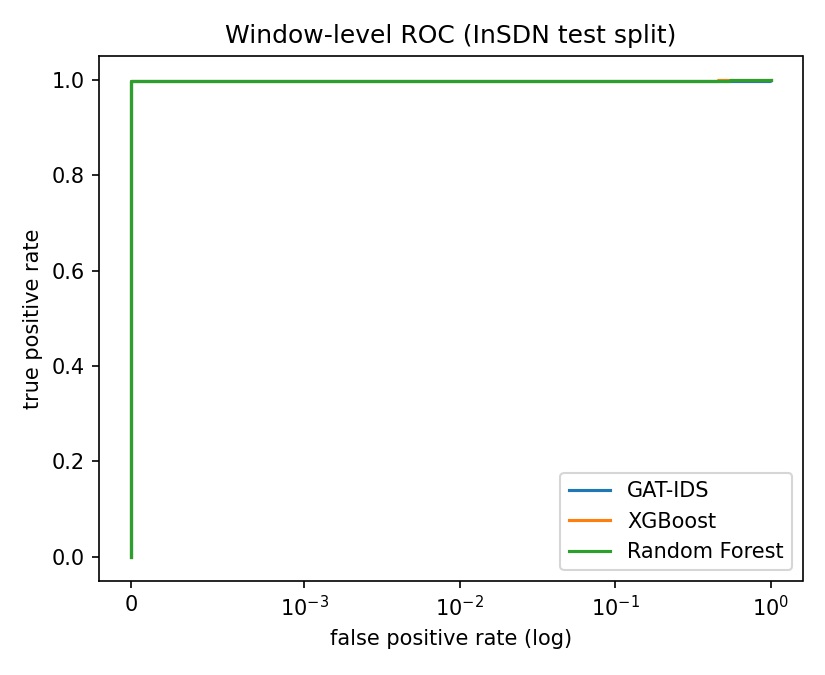
\includegraphics[width=0.75\textwidth]{roc_windows}
\caption{ROC curves of the window-level attack detection}
\label{fig:roc}
\end{figure}

\begin{figure}[htbp]
\centering
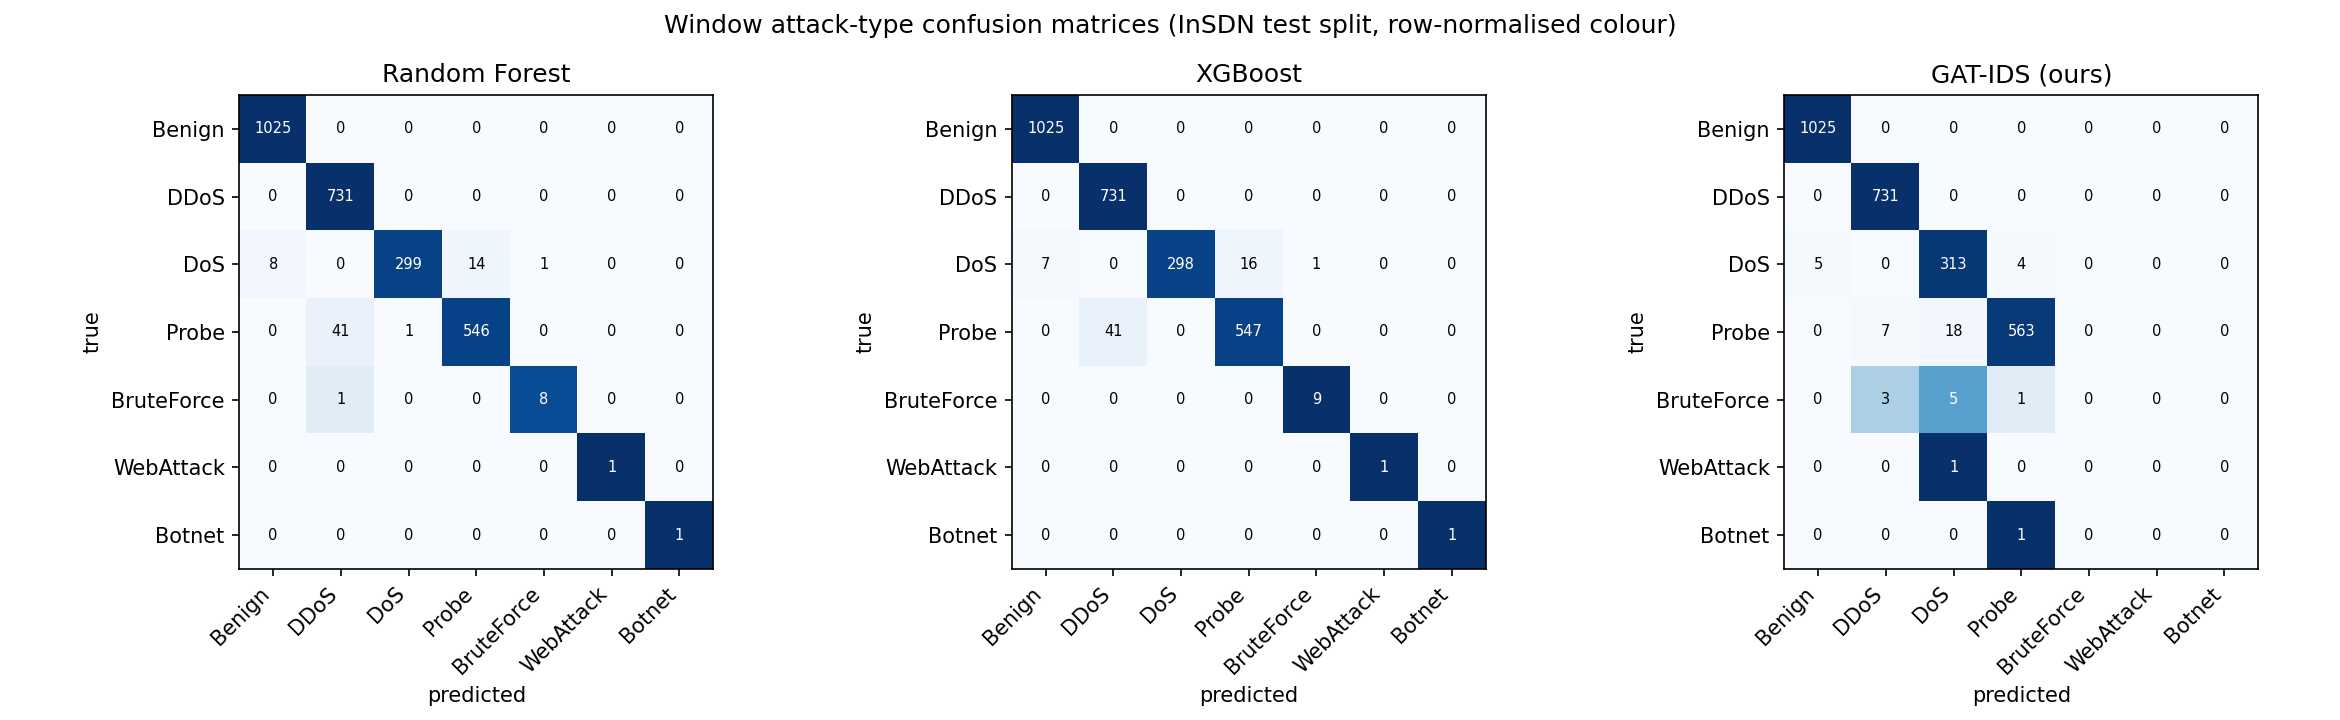
\includegraphics[width=\textwidth]{confusion_matrices}
\caption{Confusion matrices of the attack-type predictions}
\label{fig:cm}
\end{figure}

\begin{figure}[htbp]
\centering
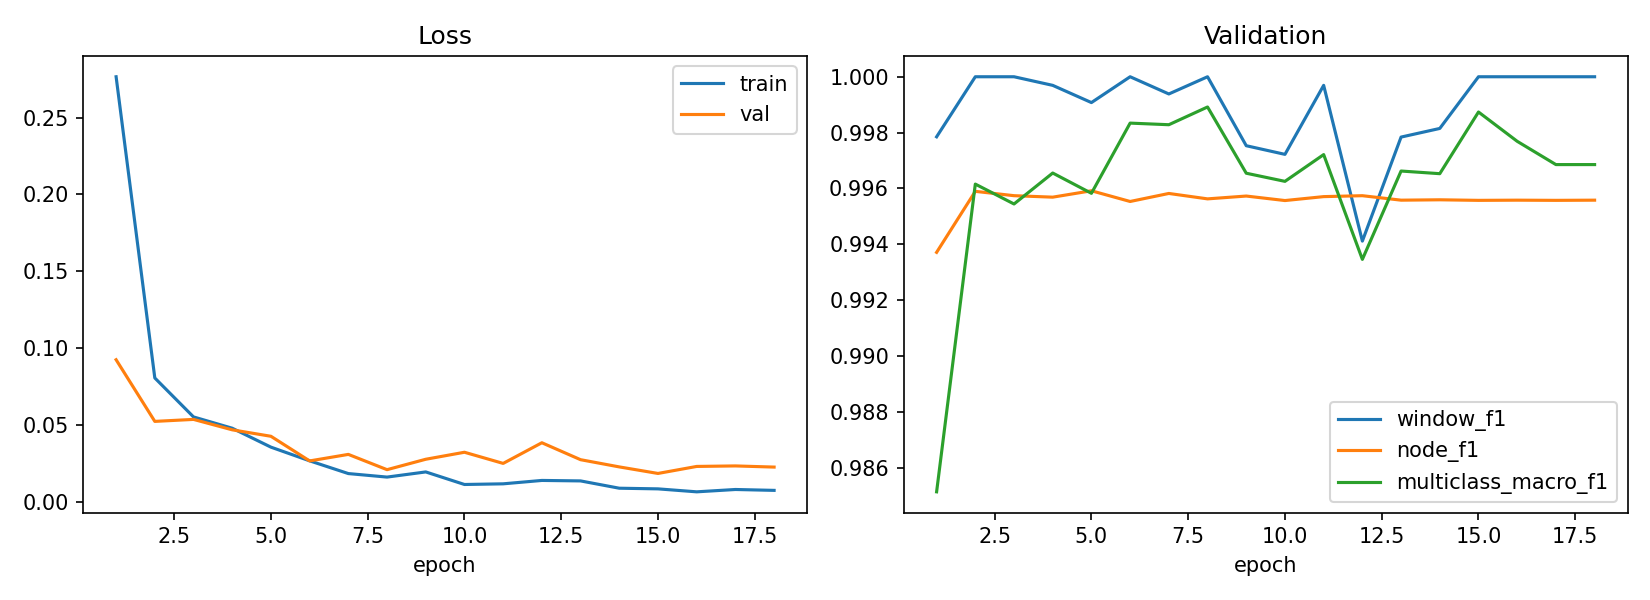
\includegraphics[width=0.85\textwidth]{gnn_v2_gat_curves}
\caption{Training and validation curves of the GAT}
\label{fig:curves}
\end{figure}

\subsection{Ablation study}

\begin{table}[htbp]
\centering
\caption{Ablation of the model (all with the 16+16 features)}
\label{tab:ablation}
\small
\begin{tabular}{|l|r|c|c|c|c|}
\hline
\textbf{Variant} & \textbf{Params} & \textbf{Window F1} & \textbf{Macro-F1 (major)} & \textbf{Host F1} & \textbf{Best epoch} \\ \hline
GAT + edge features (main) & 65,418 & 0.9985 & 0.9785 & 0.9975 & 2 \\ \hline
GCN + edge features & 56,842 & 1.0000 & 0.9837 & 0.9971 & 17 \\ \hline
GraphSAGE + edge features & 65,034 & 0.9991 & 0.9106 & 0.9984 & 24 \\ \hline
GAT without edge features & 35,402 & 0.9997 & 0.9814 & 0.9929 & 12 \\ \hline
GAT, window 50 flows & 65,418 & 0.9988 & 0.9911 & 0.9981 & 23 \\ \hline
GAT, window 200 flows & 65,418 & 1.0000 & 0.9848 & 0.9985 & 20 \\ \hline
\end{tabular}
\end{table}

The window-size variants are evaluated on their own test windows (different numbers of windows), so they cannot be compared exactly with the others.

\subsection{Feature selection and dimensionality reduction}

Table~\ref{tab:featsel} gives the main outcomes of the comparison (a Random-Forest probe on 40,000 rows; edge table: flow-level attack detection, node table: attacker host detection; the validation F1 is used for selection).

\begin{table}[htbp]
\centering
\caption{Feature-selection comparison (validation F1 / test F1 of the probe model at the $k$ with the highest validation F1)}
\label{tab:featsel}
\small
\begin{tabular}{|l|c|c|c|c|}
\hline
 & \multicolumn{2}{c|}{\textbf{Edge features (16)}} & \multicolumn{2}{c|}{\textbf{Node features (16)}} \\ \hline
\textbf{Method} & \textbf{$k$} & \textbf{Val / Test F1} & \textbf{$k$} & \textbf{Val / Test F1} \\ \hline
All features & 16 & 0.9692 / 0.9391 & 16 & 0.9968 / 0.9964 \\ \hline
ANOVA F-test & 8 & 0.9635 / 0.9164 & 8 & 0.9967 / 0.9954 \\ \hline
Mutual information & 10 & 0.9705 / 0.9350 & 10 & 0.9966 / 0.9960 \\ \hline
RF importance & 12 & 0.9528 / 0.8998 & 10 & 0.9966 / 0.9961 \\ \hline
L1 logistic & 8 & 0.9684 / 0.9327 & 12 & 0.9966 / 0.9956 \\ \hline
RFE (logistic) & 8 & 0.9684 / 0.9327 & 8 & 0.9957 / 0.9940 \\ \hline
PCA & 12 & 0.9607 / 0.9492 & 12 & 0.9959 / 0.9949 \\ \hline
Truncated SVD & 12 & 0.9607 / 0.9492 & 12 & 0.9959 / 0.9949 \\ \hline
FastICA & 8 & 0.9640 / 0.9561 & 10 & 0.9965 / 0.9958 \\ \hline
\end{tabular}
\end{table}

With a tolerance of 0.005 in validation F1, the selected subsets are: \textbf{edge} -- L1 logistic regression, $k=8$ (packets, bytes, duration, packet rate, byte rate, UDP flag, well-known destination port, well-known source port); \textbf{node} -- mutual information, $k=4$ (out-packets, out-bytes, in-bytes, mean outgoing duration). PCA and SVD give almost identical results because the features are already standardised, and the unsupervised reductions do not beat the best supervised selections on the node table. The GAT retrained on the selected subsets (64,138 parameters, best epoch 8) obtains a window F1 of 0.9976 (precision 1.0, recall 0.9952, FPR 0, ROC-AUC 0.9970) a major-class macro-F1 of 0.9868 and a host F1 of 0.9952 (precision 0.9998, recall 0.9907, FPR 0.03\%, 119,771 test hosts of which 74,808 are attackers) on the same test windows, i.e., the reduced model is comparable to the full-feature GAT of Table~\ref{tab:main} (window F1 0.9976 vs 0.9985; major-class macro-F1 0.9868 vs 0.9785; host F1 0.9952 vs 0.9975), with half as many edge features to compute. Note that the full-feature results in the other tables were produced before this retraining.

\subsection{Detection latency}

\begin{table}[htbp]
\centering
\caption{Latency per window (ms) on CPU and on the RTX 3050 GPU (selected window sizes)}
\label{tab:latency}
\small
\begin{tabular}{|l|r|c|c|c|c|}
\hline
\textbf{Device} & \textbf{Records} & \textbf{p50} & \textbf{p90} & \textbf{p99} & \textbf{GNN forward p50} \\ \hline
CPU & 100 & 3.6 & 3.9 & 4.3 & 1.1 \\ \hline
CPU & 1000 & 10.8 & 11.9 & 13.7 & 2.4 \\ \hline
CPU & 5000 & 46.5 & 48.8 & 52.3 & 15.2 \\ \hline
CPU & full service path & 6.5 & 8.7 & 9.6 & -- \\ \hline
GPU & 1000 & 9.3 & 9.9 & 11.3 & 1.9 \\ \hline
GPU & 5000 & 33.4 & 38.3 & 41.0 & 2.9 \\ \hline
GPU & full service path & 7.1 & 9.1 & 10.3 & -- \\ \hline
\end{tabular}
\end{table}

\begin{figure}[htbp]
\centering
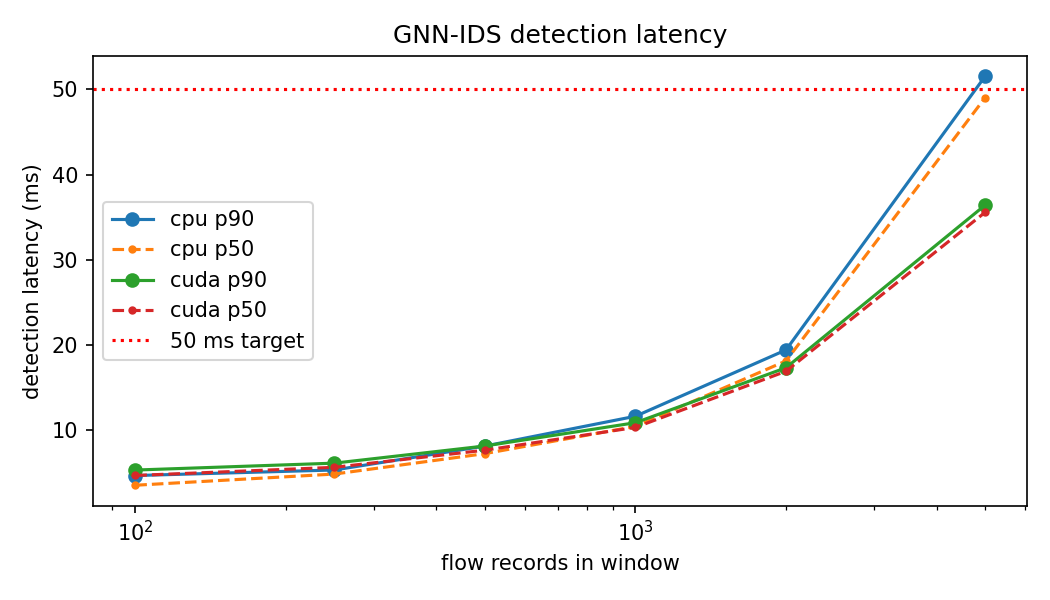
\includegraphics[width=0.8\textwidth]{latency_histogram}
\caption{Latency distribution of the IDS service}
\label{fig:latency}
\end{figure}

\subsection{Live pipeline on replayed InSDN flows}

Held-out flows were replayed to the live IDS as OpenFlow statistics (2~s polls, 10~s windows): benign, then attack mixed with benign, then benign again, for each attack type.

\begin{table}[htbp]
\centering
\caption{Replay of held-out flows through the live path}
\label{tab:replay}
\small
\begin{tabular}{|l|c|l|c|l|}
\hline
\textbf{Attack} & \textbf{Windows flagged} & \textbf{Predicted types} & \textbf{Attacker IPs blocked} & \textbf{Rule action} \\ \hline
DDoS & 10/10 & DDoS 10 & 0\% (victim protected) & rate-limit \\ \hline
DoS & 10/10 & DoS 10 & 100\% & drop \\ \hline
Probe & 10/10 & Probe 10 & 100\% & -- \\ \hline
BruteForce & 10/10 & BruteForce 8, Botnet 2 & 50\% & -- \\ \hline
\end{tabular}
\end{table}

There were no false alerts in 55 benign windows (FPR 0\%), and no benign-only address was blocked. The latency of the complete live path was 14.1~ms (p50) and 23.1~ms (p99).

\subsection{Live results in the Mininet laboratory}

The model trained only on InSDN does not transfer to the laboratory: on 2,301 held-out lab windows its window F1 is 0.6914 with an FPR of 0.9869, because the benign laboratory traffic (three clients polling one web server and an iperf stream) looks different from the benign InSDN capture. After fine-tuning on separately recorded lab runs (split by run), the same measurement gives F1 0.9958 and FPR 0.0169, with no loss on InSDN (Table~\ref{tab:finetune}).

\begin{table}[htbp]
\centering
\caption{Transfer to the laboratory and effect of fine-tuning}
\label{tab:finetune}
\small
\begin{tabular}{|l|c|c|c|c|}
\hline
\textbf{Model and test data} & \textbf{Window F1} & \textbf{FPR} & \textbf{Macro-F1 (major)} & \textbf{Host F1} \\ \hline
InSDN-only model, lab test (2,301 windows) & 0.6914 & 0.9869 & 0.1644 & 0.9373 \\ \hline
Fine-tuned model, lab test & 0.9958 & 0.0169 & 0.9943 & 0.9999 \\ \hline
InSDN-only model, InSDN test & 0.9985 & 0.0000 & 0.9785 & 0.9975 \\ \hline
Fine-tuned model, InSDN test & 0.9982 & 0.0000 & 0.9905 & 0.9987 \\ \hline
\end{tabular}
\end{table}

The mitigation logic was developed in four iterations, each driven by a problem found in the live runs (Table~\ref{tab:mitigation}; 12 runs per version except the first).

\begin{table}[htbp]
\centering
\caption{Live mitigation: effect of each design change}
\label{tab:mitigation}
\small
\begin{tabularx}{\textwidth}{|X|c|c|c|c|}
\hline
\textbf{Version} & \textbf{Mitigated} & \textbf{Runs with benign host blocked} & \textbf{Mean attack traffic dropped} & \textbf{Runs $\ge 70\%$} \\ \hline
Initial, InSDN-only model (1 DoS run) & 1/1 & 1 & 100\% & 1/1 \\ \hline
Fine-tuned, max host score, kbit/s meters, no persistence & 12/12 & 9 & 75.6\% & 8/12 \\ \hline
+ mean host score, 2-window persistence, packet/s meters & 12/12 & 1 & 65.7\% & 6/12 \\ \hline
\textbf{Final: + rule priorities by severity, per-switch tracking} & \textbf{12/12} & \textbf{0} & \textbf{94.7\%} & \textbf{12/12} \\ \hline
\end{tabularx}
\end{table}

\begin{table}[htbp]
\centering
\caption{Final system: results by attack scenario (3 runs each)}
\label{tab:final}
\small
\begin{tabular}{|l|c|c|c|c|}
\hline
\textbf{Scenario} & \textbf{Mitigated} & \textbf{Mean drop rate} & \textbf{Mean time to mitigation} & \textbf{Benign traffic to victim kept} \\ \hline
BruteForce & 3/3 & 100.0\% & 4.5 s & 121.1\%$^{*}$ \\ \hline
DDoS & 3/3 & 79.9\% & 3.9 s & 3.0\% \\ \hline
DoS & 3/3 & 100.0\% & 4.4 s & 98.1\% \\ \hline
Probe & 3/3 & 98.9\% & 17.4 s & 96.3\% \\ \hline
\end{tabular}

{\footnotesize $^{*}$ The value is a ratio to a reference period and can exceed 100\%; it means that legitimate traffic was not reduced.}
\end{table}

\begin{figure}[htbp]
\centering
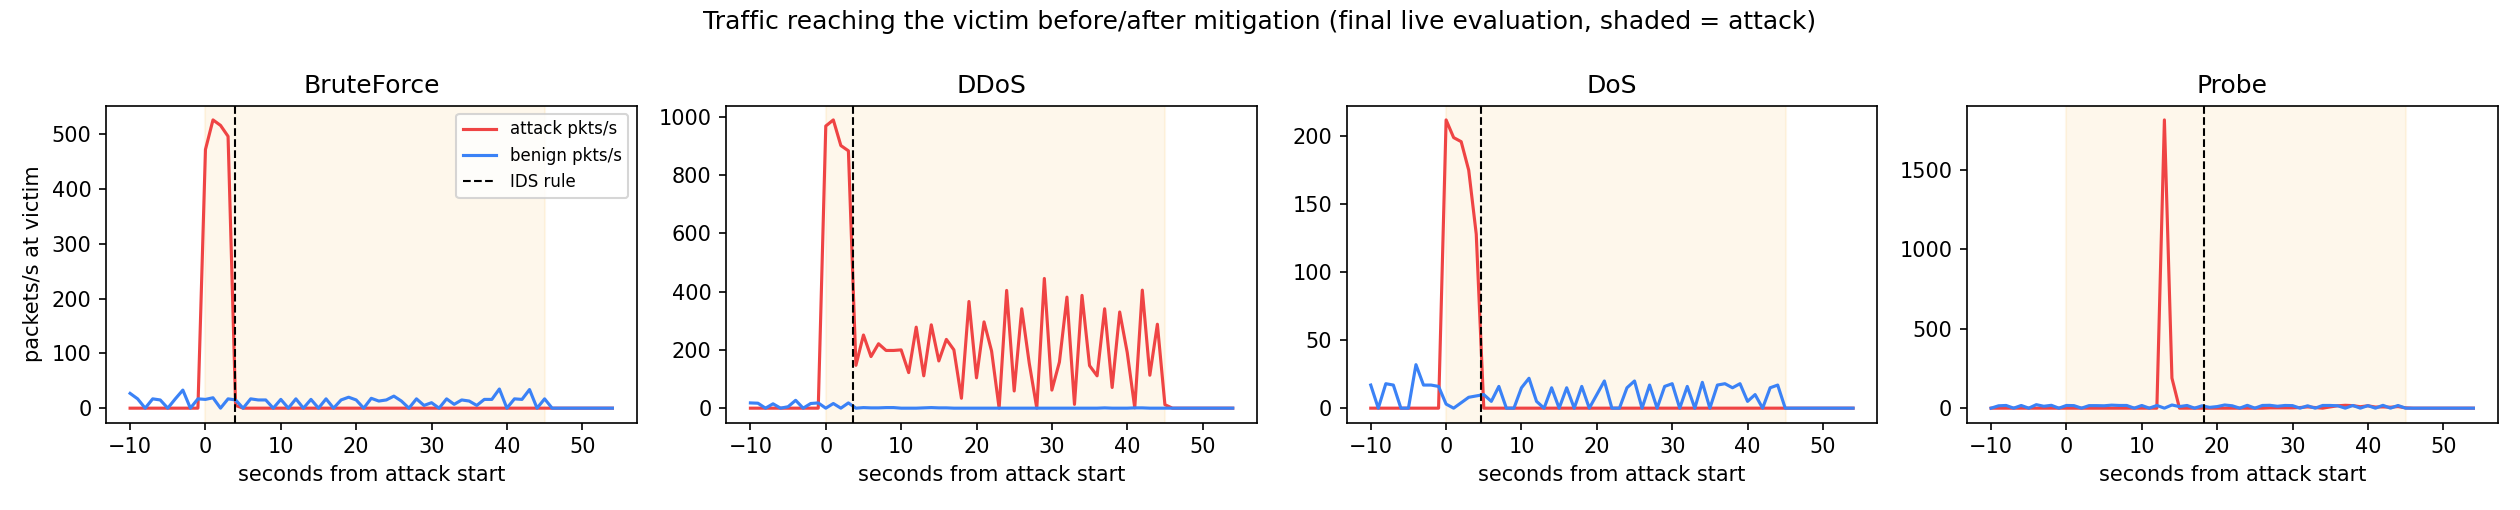
\includegraphics[width=\textwidth]{mitigation_timeline}
\caption{Timeline of a mitigated attack: traffic to the victim and the moment the rule is installed}
\label{fig:timeline}
\end{figure}

\begin{figure}[htbp]
\centering
\fbox{\parbox{0.9\textwidth}{\centering\vspace{2cm}\textit{Insert screenshot of the offline results dashboard (\texttt{/}) here}\vspace{2cm}}}
\caption{Offline results dashboard}
\label{fig:shot-offline}
\end{figure}

\begin{figure}[htbp]
\centering
\fbox{\parbox{0.9\textwidth}{\centering\vspace{2cm}\textit{Insert screenshot of the live monitor (\texttt{/live}) during a DDoS run here}\vspace{2cm}}}
\caption{Live monitor showing the traffic graph, alerts and active rules}
\label{fig:shot-live}
\end{figure}


\subsection{Per-Run Results of the Final System}
Table~\ref{tab:perrun} gives the individual results of the 12 attack runs behind Table~\ref{tab:final}. ``Attack pps'' is the packet rate of the attack traffic measured at the victim link before the first rule and after it, and ``Benign pps'' is the same for the benign traffic to the victim.

\begin{table}[htbp]
\centering
\caption{Individual live attack runs (final system)}
\label{tab:perrun}
\small
\begin{tabular}{|l|c|c|c|c|c|c|}
\hline
\textbf{Attack} & \textbf{Run} & \textbf{Time to rule (s)} & \textbf{Attack pps before} & \textbf{Attack pps after} & \textbf{Drop rate} & \textbf{Benign pps before / after} \\ \hline
DDoS & 1 & 3.6 & 988 & 200 & 79.8\% & 9.5 / 0.4 \\ \hline
DoS & 1 & 4.6 & 196 & 0 & 100.0\% & 10.0 / 9.6 \\ \hline
Probe & 1 & 18.2 & 390 & 5 & 98.6\% & 10.9 / 10.8 \\ \hline
BruteForce & 1 & 4.0 & 504 & 0 & 100.0\% & 10.5 / 12.1 \\ \hline
DDoS & 2 & 3.8 & 987 & 200 & 79.8\% & 11.2 / 0.4 \\ \hline
DoS & 2 & 5.0 & 197 & 0 & 100.0\% & 9.6 / 10.2 \\ \hline
Probe & 2 & 16.6 & 567 & 5 & 99.1\% & 11.2 / 9.5 \\ \hline
BruteForce & 2 & 4.4 & 526 & 0 & 100.0\% & 8.8 / 13.0 \\ \hline
DDoS & 3 & 4.1 & 987 & 198 & 80.0\% & 8.4 / 0.1 \\ \hline
DoS & 3 & 3.8 & 201 & 0 & 100.0\% & 11.6 / 10.8 \\ \hline
Probe & 3 & 17.2 & 481 & 6 & 98.8\% & 9.2 / 9.8 \\ \hline
BruteForce & 3 & 5.0 & 525 & 0 & 100.0\% & 9.4 / 9.7 \\ \hline
\end{tabular}
\end{table}

Three observations follow from the table. First, the runs of one scenario are very similar (time to mitigation of DoS between 3.8 and 5.0~s, drop rate 100\% in all three), so the results are stable and not due to a lucky run. Second, the DDoS drop rate of 79.8--80.0\% is the same in all runs because it is fixed by the limiter: the flood of about 988 packets/s is cut to the 200 packets/s of the victim rate limit, i.e., $1-200/988\approx0.80$; the benign traffic to the victim is cut in the same proportion (from about 10 packets/s to below 0.5 packets/s) because the meter cannot tell the packets apart. Third, the Probe runs need 16.6 to 18.2 seconds, because nmap scans of 2,000 ports are completed in a few seconds and the system needs several windows to confirm the scanner; after the rule the scan rate falls from 390--567 packets/s to about 5 packets/s.

\subsection{Latency Breakdown by Stage}
The latency was re-measured with the feature-selected model, with 200 repetitions per window size. Table~\ref{tab:latstage} gives the median time of each stage of the engine.

\begin{table}[htbp]
\centering
\caption{Median time per stage (ms) of the inference engine}
\label{tab:latstage}
\small
\begin{tabular}{|l|r|c|c|c|c|c|}
\hline
\textbf{Device} & \textbf{Records} & \textbf{Features} & \textbf{Graph} & \textbf{Model} & \textbf{Decision} & \textbf{Total} \\ \hline
CPU & 100 & 1.0 & 0.07 & 1.1 & 1.3 & 3.5 \\ \hline
CPU & 500 & 3.4 & 0.13 & 1.8 & 1.7 & 7.2 \\ \hline
CPU & 1000 & 5.8 & 0.17 & 2.3 & 2.0 & 10.4 \\ \hline
CPU & 2000 & 11.3 & 0.25 & 3.6 & 2.8 & 18.1 \\ \hline
CPU & 5000 & 27.8 & 0.47 & 15.9 & 4.7 & 49.0 \\ \hline
GPU & 100 & 1.0 & 0.23 & 2.1 & 1.3 & 4.7 \\ \hline
GPU & 500 & 3.3 & 0.30 & 2.4 & 1.7 & 7.6 \\ \hline
GPU & 1000 & 5.7 & 0.33 & 2.3 & 2.0 & 10.3 \\ \hline
GPU & 2000 & 11.3 & 0.43 & 2.5 & 2.6 & 16.9 \\ \hline
GPU & 5000 & 27.6 & 0.55 & 2.9 & 4.4 & 35.6 \\ \hline
\end{tabular}
\end{table}

The table shows that the neural network is \emph{not} the main cost. At 1,000 records the feature computation takes 5.8~ms and the model 2.3~ms; at 5,000 records the feature computation is 27.8~ms on both devices, while the model needs 15.9~ms on the CPU and 2.9~ms on the GPU. The GPU therefore only helps for very large windows. The feature computation is done in pandas and NumPy and is the part to optimise first if larger windows must be handled. In the same measurement the complete service path (HTTP request, collector, engine, classifier, mitigation, response) had a median of 7.1~ms and a 99th percentile of 10.3~ms on the CPU, and 8.0~ms and 10.7~ms on the GPU, for polls of 60 flows; the replay of held-out flows (on average 274 flows per window) had a median of 8.0~ms and a 99th percentile of 13.7~ms. These values are consistent with Table~\ref{tab:latency}.

\subsection{Training Behaviour}
Figure~\ref{fig:curves} shows the loss and the validation scores per epoch of the final training run. The training loss decreases from 0.277 to 0.007 over the 18 epochs that were run, while the validation loss decreases from 0.092 to 0.021 and then fluctuates between 0.018 and 0.038. The validation window F1 is already 0.998 after the first epoch and stays between 0.994 and 1.0, and the node F1 is constant at 0.9956--0.9959 after the second epoch. The major-class macro-F1 on the validation set rises from 0.985 to 0.999 at epoch 8, which is the epoch that was selected. Two conclusions follow. The task is learned very quickly, in line with the regularity of the dataset; and since the validation scores fluctuate by a few tenths of a percent from epoch to epoch while the training loss continues to fall, the model starts to over-fit after about 8 epochs, which early stopping with a patience of 10 handles.

\subsection{Replay Experiment in Detail}
The replay script cuts held-out flows by attack type and replays them in real time: 15 polls (30~s) of benign traffic with 20 flows per poll, then 10 polls (20~s) of attack traffic with 40 flows per poll mixed with the benign flows, then benign traffic again; the poll interval is 2~s. Table~\ref{tab:replaydetail} shows the outcome by attack type. The attack was detected in the first attack window in all four cases (detection delay 0~s), because the replay uses 2-window confirmation only for blocking, not for the alert. The DDoS replay contained 400 spoofed attacker addresses; the engine created a single rate-limit rule for the victim (192.168.20.134) instead of 400 rules, and the DoS replay created one drop rule for the single attacker. For Probe and BruteForce, the report records no rule created in the replay; the reason was not analysed in detail, and the attacker coverage values (100\% and 50\%) are those of the report.

\begin{table}[htbp]
\centering
\caption{Replay of held-out flows through the live path}
\label{tab:replaydetail}
\small
\begin{tabular}{|l|c|c|c|c|c|}
\hline
\textbf{Attack} & \textbf{Windows flagged} & \textbf{True attacker IPs} & \textbf{Rules created} & \textbf{Attacker coverage} & \textbf{False blocks} \\ \hline
DDoS & 10/10 & 400 & 1 (victim rate limit) & 0\% (by design) & none \\ \hline
DoS & 10/10 & 1 & 1 (drop) & 100\% & none \\ \hline
Probe & 10/10 & 1 & 0 & 100\% & none \\ \hline
BruteForce & 10/10 & 2 & 0 & 50\% & none \\ \hline
\end{tabular}
\end{table}

Among the benign polls there were 55 windows with no false alert and no suspicious window; one source address was blocked in the whole experiment, and it was an attacker address; the 111 addresses that appeared only in benign traffic were never blocked.

\section{Analysis}

\subsection{Comparison with the Project Targets}
Table~\ref{tab:targets} compares the measured results with the targets that were set at the start of the project (architecture document, performance targets).

\begin{table}[htbp]
\centering
\caption{Targets and results}
\label{tab:targets}
\small
\begin{tabularx}{\textwidth}{|p{3.6cm}|p{3.4cm}|p{3.6cm}|X|}
\hline
\textbf{Metric} & \textbf{Target} & \textbf{Result} & \textbf{Met?} \\ \hline
F1 gain over XGBoost on coordinated attacks & +15--25\% & Macro-F1 0.9785 vs 0.9703; error 3.0\% $\to$ 2.2\%; binary F1 $\ge 0.997$ for all models & Partly: the baseline is already at 0.97, so a relative gain of this size is impossible \\ \hline
Inference latency & $<50$~ms per window & Service path p90 8.7~ms, p99 9.6~ms (CPU) & Yes \\ \hline
Attack traffic dropped & $\ge 70\%$ & 12/12 runs, mean 94.7\% & Yes \\ \hline
Time to mitigation & Within two controller round-trips (about 100~ms) & Median 4.5~s, mean 7.5~s & No: limited by 2~s polling, 10~s window and two-window confirmation \\ \hline
False-positive rate & $<5\%$ & 0\% on InSDN test; 1.7\% of benign lab windows; 0 benign hosts blocked in 12 attack runs; 0 rules in benign-only runs & Yes \\ \hline
\end{tabularx}
\end{table}

\subsection{Reading the Result Tables in Detail}
\textbf{Table~\ref{tab:main}.} Each row is one model evaluated on the same 2,677 test windows. \emph{Window F1} measures whether the window is an attack (the positive class has 1,652 windows); \emph{FPR} is the share of the 1,025 benign windows that were wrongly flagged, and it is zero for all three. \emph{ROC-AUC} is slightly higher for the tree models (0.9987) than for the GAT (0.9982), which shows that the GAT does not rank windows better; its advantage lies in the choice of the threshold and in the typed and host decisions. \emph{Macro-F1 (major)} averages the F1 of Benign, DDoS, DoS and Probe, and \emph{Host F1} is computed over all hosts of all windows.\\

\textbf{Table~\ref{tab:perclass}.} For DDoS and Probe the GAT is clearly better (0.993 vs 0.973 and 0.973 vs 0.951), which are the two classes whose shape on the graph is most distinctive (many sources for DDoS, many ports for Probe). The DoS class is the only major class where the baselines are better (0.961 vs 0.950). The three rare classes have one to nine windows, so one wrongly classified window changes the F1 by 11 to 100 points; they are shown for completeness.\\

\textbf{Table~\ref{tab:ablation}.} The first column is the variant, the second the parameter count (the no-edge-feature model is about half as large, since it has no edge encoder), and the others the test metrics. The best-epoch column shows that all models converge quickly: the main GAT has its best validation score in epoch 2 and training continues only until the patience of 10 epochs is exhausted.\\

\textbf{Table~\ref{tab:latency}.} Rows give the number of flow records in the window. The ``GNN forward'' column is the neural-network time alone; the difference to p50 is the cost of the feature computation, graph construction and decision. The row ``full service path'' is the measurement over the real HTTP service with realistic windows.\\

\textbf{Table~\ref{tab:replay}.} ``Windows flagged'' counts the attack windows (10 per attack type) in which the IDS raised an ATTACK. ``Attacker IPs blocked'' is the share of the real attacker addresses that received a rule; for DDoS it is 0\% on purpose, because the policy protects the victim instead of blocking spoofed sources. BruteForce windows were partly typed as Botnet (2 of 10), which is a plausible confusion of two low-volume, repeated-connection classes, and half of the BruteForce attackers were blocked.\\

\textbf{Tables~\ref{tab:mitigation} and~\ref{tab:final}.} ``Mitigated'' means that at least one rule was installed during the run. ``Mean attack traffic dropped'' is measured from the packet capture at the victim at the packet capture of the victim link. The last column of Table~\ref{tab:final} gives the share of benign traffic to the victim that survived the mitigation.

\subsection{Error Analysis}
\begin{itemize}
	\item \textbf{GAT versus the baselines on rare classes.} The GAT is trained with graphs in which BruteForce, WebAttack and Botnet appear in very few windows; with class weights capped at 10 the model still does not learn them. The tree models score flows and aggregate them, so a single distinctive flow is enough to type the window.
	\item \textbf{DoS windows.} Some DoS windows are typed as Benign or BruteForce. A DoS window of 100 flows from one attacker has the same graph shape as a BruteForce window; the difference is in rates and sizes, which are weaker signals than the graph shape.
	\item \textbf{First live test.} The InSDN-only model gave an FPR of 0.987 on lab windows, which means that almost all benign lab windows looked like attacks. A likely explanation is that the model learned the InSDN benign distribution (windows of about 22 hosts) and the lab benign windows (6 hosts and a steady iperf stream) lie outside it; this was not tested separately.
	\item \textbf{Early live versions.} Blocking of benign clients was caused by decision logic and not by the model: the per-host false-positive rate was 0.38\% offline, but a host is scored about 20 times per window and a new window arrives every 2~s.
	\item \textbf{DDoS mitigation.} The remaining loss of legitimate traffic during a spoofed flood is a property of IP-based rules and not of the detector.
\end{itemize}

\subsection{Threats to Validity}
\begin{itemize}
	\item \textbf{Internal.} The test windows come from the same captures as the training windows (although separated in time with a gap), so the offline scores are optimistic about new environments; the laboratory result before fine-tuning (F1 0.69) shows how large the gap can be.
	\item \textbf{Window overlap inside a split.} Windows within the test split overlap each other (stride 25 of 100), so the 2,677 test windows are not independent samples and confidence intervals would be wider than the sample size suggests.
	\item \textbf{External.} Four attack types, one small topology and one dataset were used; the conclusions about the relative merit of GAT, GCN and GraphSAGE should not be generalised to other datasets.
	\item \textbf{Statistical.} Only one random seed (42) was used for each model, so small differences (for example 0.9985 vs 0.9991 window F1) are not significant. Twelve live runs are too few for an exact false-block rate.
	\item \textbf{Construct.} The window label rule (at least 10\% attack flows) and the direction heuristic define what counts as correct; a different rule would change the metrics.
\end{itemize}

\subsection{Reproducing the Results}
All the results of this chapter are generated by scripts that read \texttt{configs/phase2.yaml}, with a fixed seed. \texttt{bash scripts/run\_all.sh} runs cleaning, graph building, baselines, training, ablations and export with a progress page; \texttt{python scripts/replay\_flows.py} and \texttt{python scripts/benchmark\_latency.py} reproduce Tables~\ref{tab:replay} and~\ref{tab:latency}; \texttt{bash scripts/run\_phase2\_demo.sh} runs the Mininet laboratory; and \texttt{python scripts/make\_phase2\_report.py} writes the results file with all tables. Each result file records the git commit and the parameters of the run.



\subsection{Offline detection}
\begin{itemize}
	\item \textbf{Binary detection is saturated.} All models detect attack windows with F1 above 0.997 and zero false positives (Table~\ref{tab:main}). InSDN windows are very regular, so the interesting comparison is the \emph{type} and \emph{host} decision. Here the GAT is better than the best baseline on the major classes (macro-F1 0.9785 vs 0.9703) and on host F1 (0.9975 vs 0.9946). The structure of the graph is exactly what separates DDoS (many one-flow sources into one victim) from DoS (few sources with many flows) and from Probe (many ports on one host): DDoS F1 improves from 0.973 to 0.993 and Probe from 0.951 to 0.973.
	\item \textbf{The project target of a 15--25\% F1 gain is not meaningful here.} The baselines are already at about 0.97, so the possible gain is below 3 points; the measured gain is an error reduction of about 27\% (3.0\% to 2.2\%). We report this honestly: the claim of the architecture document is only partly met.
	\item \textbf{DoS is slightly worse than the baselines} (0.950 vs 0.961). The cause was not analysed in detail; in the confusion matrix of the feature-selected model the misclassified DoS windows go to Benign, BruteForce and WebAttack.
	\item \textbf{Rare classes.} BruteForce (9 test windows), WebAttack (1) and Botnet (1) are not learned by the GAT, whereas the tree models classify them. With so few windows their F1 values are noise, which is why the major-class macro-F1 is used for model selection, but it is also a real limitation: graph structure helps with volumetric and scanning attacks, not with attacks that are distinguished by application content that OpenFlow counters do not contain.
	\item \textbf{Ablations.} GCN, GraphSAGE and a GAT without edge features have similar window F1, so the ability to detect an attack does not depend on the layer type. The differences appear in the type decision (GraphSAGE 0.911 vs GAT 0.979) and in the host decision (without edge features, host F1 falls from 0.9975 to 0.9929), which shows that attention with edge features helps the attacker identification. GCN has a macro-F1 comparable to GAT (0.984), so the advantage of attention is moderate on this dataset, and we kept GAT because of the best host results and because it is the model integrated with the controller. The best epoch of the main model is early (epoch 2) with a very high validation score, which suggests that the task is easy for the model and that the validation curves are flat; this points to the regularity of the dataset rather than to a hard-won optimum.
	\item \textbf{Feature selection.} Dropping from 16 to 8 edge features and 4 node features costs little on the probe (node F1 0.9942 vs 0.9964), and the GAT trained on the reduced set is comparable to the full model, so a compact set of counters is sufficient. A caution is that the 4 selected node features are volume features; the topology information (degree, entropy) is not lost because the graph structure itself is the input of the GNN.
\end{itemize}

\subsection{Latency}
The complete service path (features, graph, model, decision) has a median of 6.5~ms and a p99 of 9.6~ms on the CPU, five times below the 50~ms target. The model forward pass itself is only 1--2~ms for typical windows. Latency grows roughly linearly with the number of flow records because windows are processed in chunks of 200; at 5,000 records the CPU p99 exceeds 50~ms (52~ms) while the GPU stays at 41~ms. The GPU is not faster for typical windows, since the fixed cost of the transfer dominates; a CPU is sufficient for deployments of this size. The warm-up at start-up is essential: without it the first calls took about 200~ms.

\subsection{Live detection and the need for fine-tuning}
The InSDN-only model flagged almost every benign laboratory window (FPR 0.987), and in the first live test it blocked benign hosts. The benign traffic of the laboratory differs from that of the dataset, so a model trained on one capture does not transfer without adaptation. Fine-tuning with labelled laboratory runs (split by run, with oversampling) removed this problem (FPR 0.017) at no cost on InSDN. This is a limitation to be aware of: a deployment will need a short calibration period with its own benign traffic.

\subsection{Mitigation}
\begin{itemize}
	\item \textbf{Final result.} All 12 attack runs were mitigated, the mean fraction of attack traffic dropped was 94.7\% with every run above 70\%, and no benign host was blocked in any run, nor in the benign-only runs (Table~\ref{tab:mitigation}).
	\item \textbf{Why the intermediate versions were worse.} (i) Taking the \emph{maximum} chunk score for a host gives a benign host about 20 chances per window to cross the threshold and 9 of 12 runs blocked a benign client; the mean score with a two-window persistence reduced this to 1 run. (ii) Measuring the rate limit in kbit/s let a SYN flood pass (the DDoS reduction was only 31\%); packets per second fixed this. (iii) With equal priorities a leftover victim rate-limit overlapped with a later drop rule for a DoS source, and DoS reduction was only 39\%; priorities by severity raised it to 100\%.
	\item \textbf{DDoS.} The drop rate of 79.9\% satisfies the target, but legitimate clients keep only 3\% of their traffic to the victim during a spoofed flood (Table~\ref{tab:final}): the 200 packets/s allowed to the victim are mostly consumed by spoofed packets. IP-based rules cannot separate spoofed from legitimate sources; protecting legitimate clients needs SYN cookies or a proxy, which is outside this project. We accept this as a limitation.
	\item \textbf{Probe.} The time to mitigation (17.4~s) is the longest, because the first complete scan is a burst of about 3~s that ends before the rule is active; the rate limit throttles the repeated scans that follow (Figure~\ref{fig:timeline}).
	\item \textbf{The ``within two controller round-trips (about 100~ms)'' target was not met.} The median time from the start of the attack to the rule is 4.5~s (mean 7.5~s). It is not limited by the model (6.5~ms) but by the architecture: the controller polls every 2~s, the window is 10~s and two consecutive windows are needed for confirmation. A shorter poll interval, or detection triggered by packet-in rates, would shorten it at the cost of more false alarms.
\end{itemize}

\subsection{Summary of the main take-away points}
\begin{enumerate}
	\item A multi-task GAT on OpenFlow-compatible graphs detects attacks at F1 0.998 with no false positives and identifies the attacker hosts at F1 0.998; it is better than the flow-level baselines on the attack-type and host decisions, but the advantage is small because the baselines are already strong on InSDN.
	\item The complete live path takes 6.5~ms per window on a CPU, so the model is not the latency bottleneck.
	\item Real SDN deployment exposed problems that the offline numbers did not show: domain shift in benign traffic, benign hosts being blocked, and unsuitable rate-limit units and rule priorities. All were corrected, and the final system dropped 94.7\% of the attack traffic with no false blocks in 12 live runs.
	\item The remaining limitations are the rare attack classes, the collateral damage during a spoofed DDoS and the multi-second reaction time.
\end{enumerate}
